En esta parte de la investigación se presentan algunos antecedentes relacionados a la detección y pre-diagnóstico de nódulos en distintos órganos y a través de diversas metodologías. Estos ayudarán a entender el enfoque y obtener bases para un correcto desarrollo del proyecto en cuestión.

%% Primer antecedente : Deep-Learning-Based Morphological Feature Segmentation for Facial Skin Image Analysis
\subsection{\citetitle{yoon2023}}

\textbf{Introducción:}
El artículo \citetitle{yoon2023}, donde \cite{yoon2023} presentan un enfoque innovador para el análisis de imágenes faciales con el objetivo de segmentar características morfológicas de la piel, como arrugas y poros, utilizando una red neuronal profunda basada en U-Net. A diferencia de los métodos tradicionales que se enfocan en el color de la piel, este método utiliza estructuras morfológicas y se integra con mecanismos de atención y codificación posicional. Esto permite una detección simultánea más precisa de arrugas y poros, un avance significativo en el campo de la dermatología estética y la industria cosmética.

\textbf{Técnicas utilizadas:}
El método propuesto utiliza una versión mejorada de la arquitectura U-Net, que incorpora esquemas de atención para enfocarse en áreas relevantes de la piel y mejorar la transmisión de características al decodificador. Se desarrollaron mapas de textura para generar la "ground truth" (GT), utilizando filtros que resaltan detalles de alta frecuencia, como bordes y coherencia para las arrugas y pirámides Laplacianas para los poros. Además, se integró información posicional para mejorar la localización de estas características y se emplearon técnicas ligeras como el "zero-padding" para reducir los falsos positivos y optimizar el rendimiento computacional.

\textbf{Metodología:}
La metodología empleada incluyó la creación de mapas de textura como "ground truth" para las arrugas y poros, lo cual refinó las anotaciones manuales mediante el uso de filtros y técnicas de análisis de imágenes. La red neuronal fue entrenada con imágenes faciales anotadas manualmente y optimizada mediante mecanismos de atención y codificación posicional. Los resultados obtenidos fueron comparados con enfoques tradicionales de procesamiento de imágenes y modelos recientes basados en aprendizaje profundo, lo que permitió evaluar la efectividad del método propuesto.

\textbf{Base de datos utilizada:}
Aunque el artículo no menciona una base de datos pública específica, se utilizaron imágenes faciales procesadas y anotadas manualmente para generar los datos de entrenamiento necesarios. Estas imágenes fueron empleadas para entrenar la red neuronal y crear los mapas de textura utilizados en la generación de la "ground truth" para las características faciales de interés, como arrugas y poros.

\textbf{Resultados:}
El enfoque propuesto mostró una segmentación precisa de arrugas y poros, como se puede ver en la Tabla \ref{tab:models_performance} y en la Figura \ref{2:fig1}, superando a los métodos tradicionales y otros modelos recientes de aprendizaje profundo en términos de precisión. La integración de mecanismos de atención mejoró significativamente la localización de las características faciales y redujo los falsos positivos. Además, la generación de la "ground truth" mediante mapas de textura demostró ser eficaz en la captura de las características morfológicas específicas de la piel facial.

\begin{table}[h!]
    \centering
    \caption{Métricas de rendimiento de diferentes modelos}
    \renewcommand{\arraystretch}{1.2} % Adjust row spacing
    \setlength{\tabcolsep}{5pt} % Adjust column spacing
    \begin{tabularx}{\textwidth}{@{}X c c c c@{}}
        \toprule
        \textbf{Models} & \textbf{\#Params} & \textbf{Loss} & \textbf{IoU of Wrinkle} & \textbf{IoU of Pore} \\ \midrule
        U-Net & 17.3 M & 1.243 & 0.2078 & 0.3601 \\
        Reduced U-Net & 4.3 M & 1.250 & 0.2147 & 0.3646 \\
        Reduced U-Net, Attentions & 5.2 M & 1.242 & 0.2250 & 0.3714 \\
        Reduced U-Net, Attentions, Zero-padding (Proposed) & 5.2 M & 1.145 & 0.2341 & 0.4032 \\ 
        \bottomrule
    \end{tabularx}
    \label{tab:models_performance}
\end{table}


\begin{figure}[!ht]
	\begin{center}
		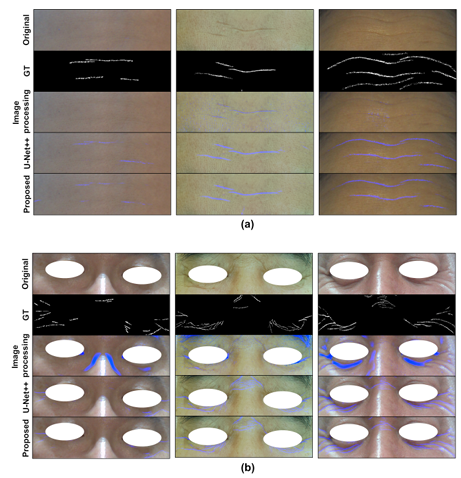
\includegraphics[width=1\textwidth]{2/figures/resant1.png}
		\caption[Comparación de la segmentación de arrugas en (a) la frente y (b) la región de los ojos]{Comparación de la segmentación de arrugas en (a) la frente y (b) la región de los ojos.\\
			Fuente: \cite{yoon2023}. \citetitle{yoon2023}. (p. 10)}
		\label{2:fig1}
	\end{center}
\end{figure}

\textbf{Conclusiones:}
Este estudio propone un avance significativo en la segmentación simultánea de arrugas y poros mediante redes neuronales profundas. El método mejora la precisión en comparación con enfoques anteriores y tiene aplicaciones potenciales en áreas como la estimación de la edad y la predicción de enfermedades cutáneas. Se sugiere que futuras investigaciones puedan ampliar esta metodología para abordar otras características faciales y problemas relacionados.

%% Segundo antecedente :  High Performing Facial Skin Problem Diagnosis with Enhanced Mask R-CNN and Super Resolution GAN
\subsection{\citetitle{Kim2023}}

\textbf{Introducción:}
El artículo de \cite{Kim2023} titulado \citetitle{Kim2023}, aborda la importancia de un diagnóstico preciso de problemas faciales de la piel, que afectan aspectos como la percepción de edad, belleza y salud. Tradicionalmente, este diagnóstico requiere visitas a clínicas especializadas, lo cual es costoso y poco práctico. Como alternativa, se propone el uso de algoritmos de aprendizaje automático para realizar diagnósticos más accesibles. Sin embargo, los enfoques basados en redes neuronales convolucionales (CNN) enfrentan desafíos técnicos, como la dificultad para detectar problemas pequeños, la identificación de hasta 20 tipos diferentes de problemas cutáneos, y la segmentación incorrecta en áreas no faciales. El objetivo del estudio es superar estas limitaciones mediante cinco tácticas específicas.

\textbf{Técnicas utilizadas:}
El estudio propone un enfoque combinado que incluye el uso de Mask R-CNN mejorado para segmentar y detectar problemas cutáneos con mayor precisión, así como Generative Adversarial Networks (GAN) para mejorar la resolución de las imágenes faciales. Además, se realizan ajustes en las redes neuronales para manejar objetos pequeños y mejorar la segmentación, así como el empleo de métodos para reducir el ruido y resaltar características relevantes en las imágenes. Se implementan técnicas para diferenciar visualmente problemas similares y mejorar la precisión en el diagnóstico.

\textbf{Metodología:}
Se entrenaron 31 modelos de segmentación utilizando las tácticas propuestas, utilizando redes preexistentes como ResNet y MobileNetV2 como base. Los modelos fueron evaluados mediante métricas como el coeficiente de similitud Dice (DSC) y se compararon con otros enfoques tradicionales basados en CNN. Esta metodología permitió evaluar la efectividad de las técnicas implementadas para superar los desafíos técnicos mencionados y mejorar el rendimiento en el diagnóstico de problemas cutáneos.

\textbf{Base de datos utilizada:}
Se emplearon 2225 fotos faciales con una resolución de 576 × 576 píxeles, que contenían diversos tipos de problemas cutáneos, como poros, lunares y acné, para entrenar y evaluar los modelos de segmentación. Estas imágenes proporcionaron un conjunto de datos diverso y representativo para evaluar la precisión del sistema en el diagnóstico de distintos problemas faciales.

\textbf{Resultados:}
El enfoque propuesto alcanzó un rendimiento del 83.38\% en el diagnóstico, superando en un 32.58\% a los métodos tradicionales basados en CNN. Además, superó a modelos como MobileNetV2, Xception y VGG19, como se ve en la Figura \ref{2:fig2}, por un promedio del 17.89\%. Uno de los logros más importantes fue la mejora significativa en la detección de objetos pequeños, como lunares, que tradicionalmente presentan baja precisión en los métodos tradicionales.

\begin{figure}[!ht]
	\begin{center}
		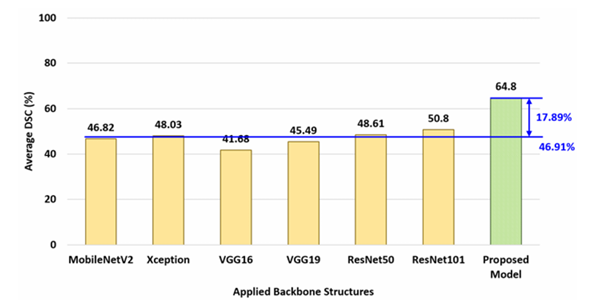
\includegraphics[width=1\textwidth]{2/figures/resultados de cuarto anteedente.png}
		\caption[Comparación del modelo propuesto con otros 6 modelos de redes neuronales]{Comparación del modelo propuesto con otros 6 modelos de redes neuronales.\\
			Fuente: \cite{Kim2023}. \citetitle{Kim2023}. (p. 8)}
		\label{2:fig2}
	\end{center}
\end{figure}

\textbf{Conclusiones:}
El sistema desarrollado, como se ve en la Figura \ref{2:fig3} demuestra ser una herramienta efectiva para diagnosticar problemas faciales de la piel con un nivel clínico de precisión, ofreciendo una alternativa viable y económica frente a las visitas a clínicas dermatológicas. Las tácticas propuestas tienen el potencial de revolucionar el cuidado facial mediante inteligencia artificial, con aplicaciones prácticas que pueden mejorar significativamente la accesibilidad y eficiencia de los diagnósticos dermatológicos.

\begin{figure}[!ht]
	\begin{center}
		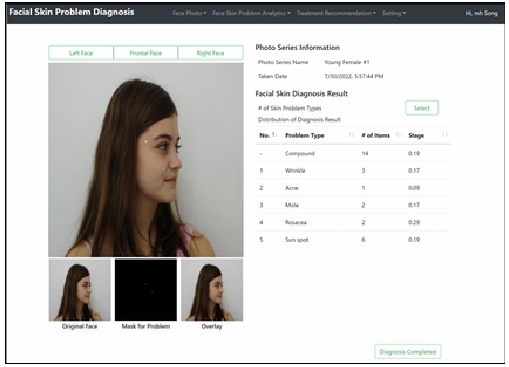
\includegraphics[width=1\textwidth]{2/figures/resant2.png}
		\caption[Interfaz de usuario del sistema de diagnóstico de problemas de la piel facial]{Interfaz de usuario del sistema de diagnóstico de problemas de la piel facial.\\
			Fuente: \cite{Kim2023}. \citetitle{Kim2023}. (p. 15)}
		\label{2:fig3}
	\end{center}
\end{figure}



%% Tercer antecedente:
\subsection{\citetitle{Zhong2024}}

\textbf{Introducción:}
El artículo titulado \citetitle{Zhong2024} de \cite{Zhong2024} presenta un enfoque innovador para la detección de arrugas faciales, abordando las limitaciones de métodos tradicionales que se ven afectados por interferencias con otras características faciales. Para mejorar la precisión, los autores proponen el uso del modelo DeepLabV3+ junto con una estrategia de etiquetado semi-automática, lo que permite generar datos de entrenamiento más representativos y mejorar la segmentación de arrugas.

\textbf{Técnicas utilizadas:}
La investigación, como podemos ver en las Figuras \ref{2:fig4} y \ref{2:fig5}, emplea técnicas avanzadas como DeepLabV3+, una red optimizada para segmentación de imágenes, y MobileNetV2 para reducir la carga computacional. Además, se desarrolla una estrategia de etiquetado semi-automática combinando anotaciones dermatológicas con mapas de textura generados mediante filtros Wiener y umbralización adaptativa. La precisión del modelo se evalúa mediante el Índice de Similitud Jaccard (JSI).

\begin{figure}[!ht]
	\begin{center}
		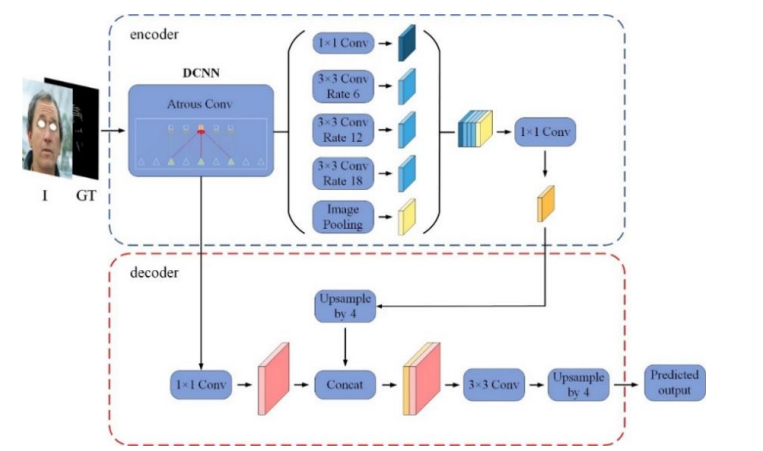
\includegraphics[width=1\textwidth]{2/figures/Meto1.png}
		\caption[Estructura de red de DeepLabV3+]{Estructura de red de DeepLabV3+.\\
			Fuente: \cite{Zhong2024}. \citetitle{Zhong2024}. (p. 4)}
		\label{2:fig4}
	\end{center}
\end{figure}


\begin{figure}[!ht]
	\begin{center}
		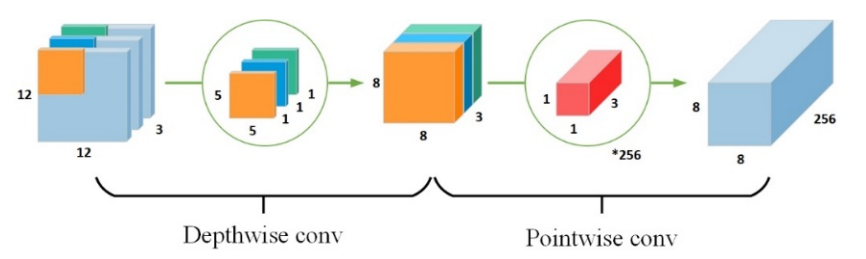
\includegraphics[width=0.80\textwidth]{2/figures/Meto2.png}
		\caption[El proceso de convolución separable en profundidad]{El proceso de convolución separable en profundidad.\\
			Fuente: \cite{Zhong2024}. \citetitle{Zhong2024}. (p. 4)}
		\label{2:fig5}
	\end{center}
\end{figure}


\textbf{Metodología:}
Se seleccionaron 300 imágenes faciales del conjunto Flickr-Face-HQ, con una resolución de 1024x1024 píxeles, para crear el conjunto de datos. Se generaron etiquetas ground truth utilizando la estrategia semi-automática propuesta. El conjunto de datos se dividió en 225 imágenes para entrenamiento, 25 para validación y 50 para pruebas. La configuración experimental incluyó un hardware con una CPU Intel Core i9-12900K, GPU RTX 3070, y 32 GB de RAM, además de utilizar el framework PyTorch para el desarrollo del modelo.

\textbf{Base de datos utilizada:}
El conjunto de datos utilizado fue el Flickr-Face-HQ, que contiene imágenes faciales de alta resolución. Este conjunto de imágenes se procesó para generar etiquetas ground truth específicas para la detección de arrugas utilizando la estrategia semi-automática propuesta.

\textbf{Resultados:}
Los resultados demostraron que el método propuesto supera a enfoques tradicionales como el filtro Hessiano y el modelo U-Net, obteniendo mayores valores de JSI en la frente (0.62) y área ocular (0.64). Además, redujo la cantidad de falsos positivos y mejoró la segmentación de bordes, logrando un mejor desempeño en la detección de arrugas finas.

\textbf{Conclusiones:}
En conclusión, el modelo DeepLabV3+ con etiquetado semi-automático se mostró más efectivo en la detección de arrugas faciales. Sin embargo, aún enfrenta desafíos en la diferenciación de arrugas muy finas y cabellos, lo que sugiere la necesidad de mejoras futuras para incrementar la precisión del sistema.


%% Cuarto antecedente: 
\subsection{\citetitle{karshiev2020improved}}

\textbf{Introducción:}
En el artículo de \cite{karshiev2020improved} llamado \citetitle{karshiev2020improved} analiza el problema de la segmentación de lesiones cutáneas, una tarea fundamental para el diagnóstico temprano del melanoma. Aunque el modelo U-Net ha sido ampliamente utilizado en segmentación médica, presenta limitaciones como ralentización en el entrenamiento y problemas con la función de activación ReLU. Para mejorar su desempeño, los autores proponen una versión optimizada que incorpora interpolación bilineal para el upsampling y la función de activación PReLU, lo que mejora la precisión y evita problemas como el sobreajuste.

\textbf{Técnicas utilizadas:}
La investigación emplea un diagrama el cual se puede ver en la Figura \ref{2:fig6} y a su vez varias técnicas clave: la interpolación bilineal sustituye la deconvolución tradicional para mejorar la segmentación de bordes, la función PReLU reemplaza ReLU para prevenir "neuronas muertas" y optimizar la convergencia, y el dropout se utiliza después de cada bloque convolucional para reducir el sobreajuste. Estas modificaciones permiten mejorar la estabilidad y eficiencia del entrenamiento.

\begin{figure}[!ht]
	\begin{center}
		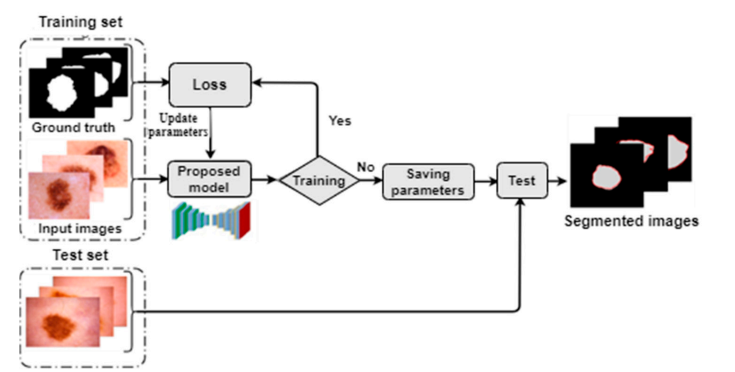
\includegraphics[width=0.80\textwidth]{2/figures/flowchart.png}
		\caption[Diagrama de flujo del sistema propuesto]{Diagrama de flujo del sistema propuesto.\\
			Fuente: \cite{karshiev2020improved}. \citetitle{karshiev2020improved}. (p. 4)}
		\label{2:fig6}
	\end{center}
\end{figure}

\textbf{Metodología:}
El modelo propuesto como se ve en la Figura \ref{2:fig7}, se basa en una arquitectura U-Net modificada con capas convolucionales optimizadas, PReLU, dropout y upsampling mediante interpolación bilineal. Fue entrenado en un sistema con un procesador Intel Core i7-9700K, 32 GB de RAM y una GPU NVIDIA GeForce RTX 2060 SUPER, garantizando un entorno adecuado para el procesamiento intensivo de imágenes médicas.

\begin{figure}[!ht]
	\begin{center}
		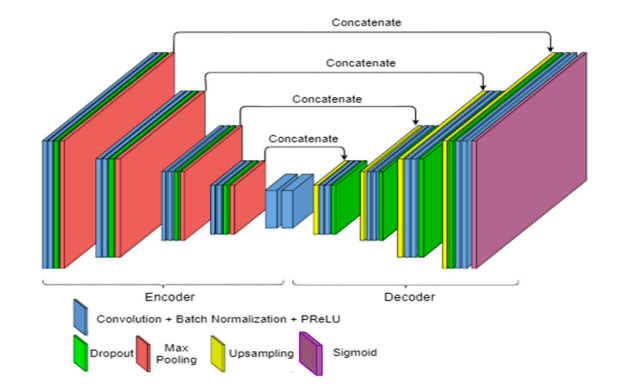
\includegraphics[width=0.80\textwidth]{2/figures/segmentation1.png}
		\caption[Modelo totalmente convolucional propuesto para la segmentación de lesiones cutáneas]{Modelo totalmente convolucional propuesto para la segmentación de lesiones cutáneas.\\
			Fuente: \cite{karshiev2020improved}. \citetitle{karshiev2020improved}. (p. 4)}
		\label{2:fig7}
	\end{center}
\end{figure}

\textbf{Base de datos utilizada:}
Para el entrenamiento y prueba del modelo se utilizó un conjunto de datos de imágenes dermoscópicas, con 2594 imágenes etiquetadas para entrenamiento y 1000 para prueba. Todas las imágenes fueron preprocesadas, redimensionadas a 256×256 píxeles y convertidas a escala de grises, lo que facilitó la normalización y mejoró la eficiencia del modelo.

\textbf{Resultados:}
Los resultados muestran un alto rendimiento del modelo mejorado, alcanzando una precisión por píxel del 94\% y un coeficiente Dice del 88\%. Estas mejoras permiten reducir artefactos en la segmentación y aumentar la eficiencia computacional en comparación con la U-Net estándar, consolidándose como una alternativa más precisa y robusta para la segmentación de lesiones cutáneas.

\textbf{Conclusiones:}
En conclusión, la versión mejorada de U-Net supera las limitaciones del modelo original al abordar problemas como gradientes débiles y artefactos en la segmentación. La integración de interpolación bilineal, PReLU y dropout permite lograr una mayor precisión y eficiencia, posicionando este enfoque como una herramienta prometedora para la segmentación de imágenes médicas en el ámbito dermatológico.

%% Quinto antecedente:
\subsection{\citetitle{Tamilkodi2024}}

\textbf{Introducción:}
\cite{Tamilkodi2024} elaboraron el artículo titulado \citetitle{Tamilkodi2024}, que presenta un software avanzado para el análisis de la piel facial que permite identificar características clave como arrugas, poros, manchas y textura, además de predecir edad y género. El sistema compara los resultados con datos de personas del mismo grupo etario, clasifica el tono de piel, genera máscaras visuales para resaltar zonas específicas del rostro y ofrece recomendaciones personalizadas. El objetivo central es desarrollar un modelo robusto capaz de realizar un análisis facial completo en diversos contextos.  

\textbf{Técnicas utilizadas:}
Para lograrlo, el software utiliza redes neuronales convolucionales profundas (D-CNN), apoyadas por modelos preentrenados para la detección de edad y género. También emplea técnicas como KMeans para clasificar el tono de piel y gradientes de Sobel para identificar arrugas. Estas herramientas se integran para ofrecer un análisis visual y cuantitativo de cada característica facial.  

\textbf{Metodología:}
La metodología del sistema incluye la captura de imágenes faciales desde múltiples ángulos, el preprocesamiento mediante técnicas como desenfoque gaussiano y conversión de formatos, seguido del análisis específico de textura, tono y arrugas. Finalmente, los resultados se visualizan en gráficos y máscaras y se utilizan para generar recomendaciones personalizadas para el usuario.  

\textbf{Base de datos utilizada:}
Como base de datos, se empleó la Indian Face Age Database (IFAD), compuesta por 3,296 imágenes de 55 personas con diversidad de edad, poses, expresiones e iluminación. Esta variedad permite entrenar modelos con mayor capacidad de generalización y robustez en escenarios reales de análisis facial.  

\textbf{Resultados:}
Los resultados como se pueden ver en las Figuras \ref{2:fig8}, \ref{2:fig9} y \ref{2:fig10} ,muestran una alta precisión en la detección de características faciales y predicciones fiables de edad y género. Además, el sistema logra una visualización efectiva mediante gráficos y máscaras que resaltan áreas clave del rostro, lo que mejora la comprensión de los resultados.  

\begin{figure}[!ht]
	\begin{center}
		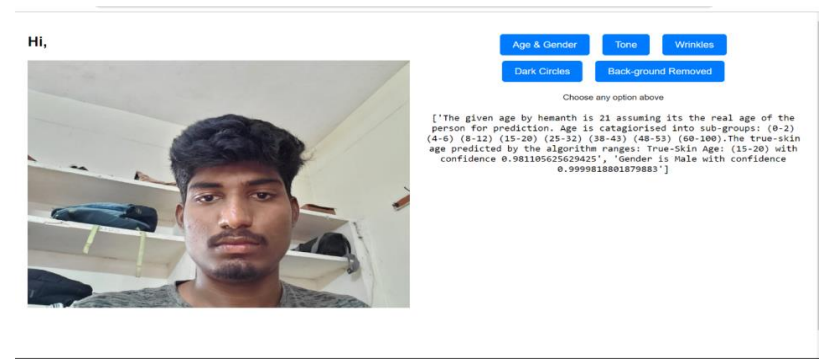
\includegraphics[width=1\textwidth]{2/figures/softres1.png}
		\caption[Detección de edad y género]{Detección de edad y género.\\
			Fuente: \cite{Tamilkodi2024}. \citetitle{Tamilkodi2024}. (p. 6)}
		\label{2:fig8}
	\end{center}
\end{figure}

\begin{figure}[!ht]
	\begin{center}
		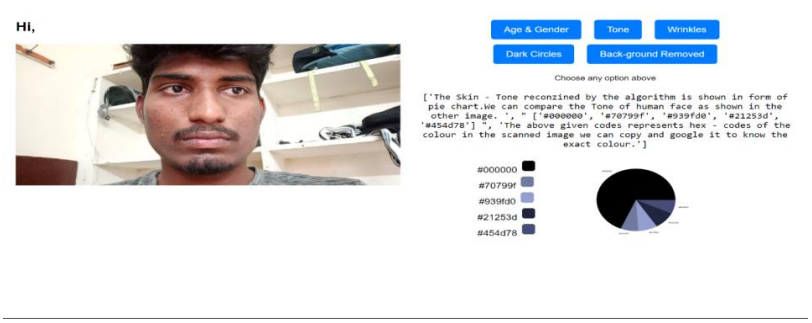
\includegraphics[width=1\textwidth]{2/figures/softres2.png}
		\caption[Análisis del tono de piel]{Análisis del tono de piel.\\
			Fuente: \cite{Tamilkodi2024}. \citetitle{Tamilkodi2024}. (p. 6)}
		\label{2:fig9}
	\end{center}
\end{figure}

\begin{figure}[!ht]
	\begin{center}
		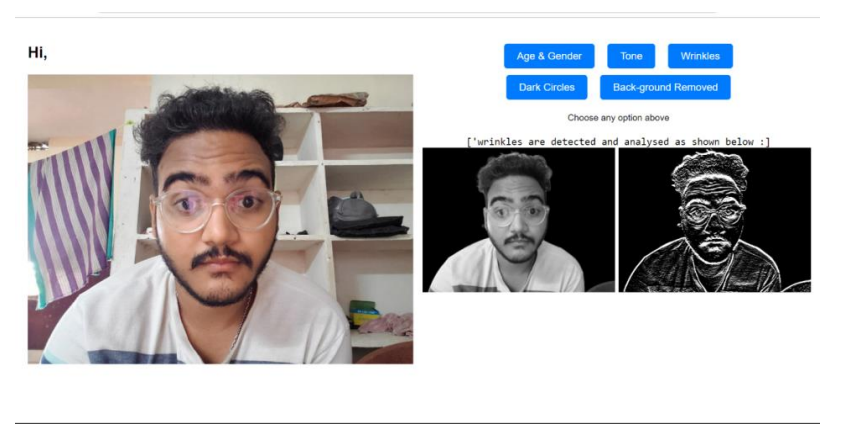
\includegraphics[width=1\textwidth]{2/figures/softres3.png}
		\caption[Análisis de arrugas]{Análisis de arrugas.\\
			Fuente: \cite{Tamilkodi2024}. \citetitle{Tamilkodi2024}. (p. 6)}
		\label{2:fig10}
	\end{center}
\end{figure}

\textbf{Conclusiones:}
En conclusión, el enfoque propuesto demuestra ser eficaz para detectar estructuras faciales importantes incluso en condiciones variables. Aunque aún no alcanza una precisión perfecta, se reconoce el valor de expandir el conjunto de datos para mejorar el rendimiento. Este modelo tiene un gran potencial para aplicaciones automatizadas en análisis dermatológico y cuidado personalizado de la piel.

%% Sexto antecedente:
\subsection{\citetitle{moon2024dermatology}}

\textbf{Introducción:}
El artículo de \cite{moon2024dermatology} llamado \citetitle{moon2024dermatology} se enfoca en la detección automática de arrugas faciales, un tema relevante en dermatología estética, debido a que los métodos manuales de segmentación son subjetivos, costosos y laboriosos. Para abordar este problema, los autores desarrollan un enfoque basado en aprendizaje profundo que incluye la creación del primer conjunto de datos público especializado en segmentación de arrugas (FFHQ-Wrinkle), y una estrategia de entrenamiento en dos etapas que combina un preentrenamiento débilmente supervisado con un ajuste fino supervisado, optimizando así el rendimiento del modelo con un uso eficiente de los recursos de etiquetado.

\textbf{Técnicas utilizadas:}
Se aplican dos enfoques complementarios: primero, un preentrenamiento débilmente supervisado que genera automáticamente mapas de textura mediante filtros Gaussianos sobre 50,000 imágenes no etiquetadas; y segundo, un ajuste fino supervisado que utiliza 1,000 imágenes con máscaras de arrugas anotadas manualmente por expertos. Para la segmentación se emplean arquitecturas de redes neuronales como U-Net y Swin UNETR, que permiten capturar tanto características locales como globales de las arrugas faciales.

\textbf{Metodología:}
La metodología, como podemos ver en la Figura \ref{2:fig11}, consiste en generar etiquetas débiles mediante mapas de textura derivados de imágenes faciales, eliminando regiones no relevantes con un modelo de segmentación facial (BiSeNet). Luego, tres expertos generan manualmente máscaras de arrugas en regiones específicas como la frente y las líneas nasolabiales. El modelo se entrena en dos etapas: primero aprende a predecir texturas con pérdida MSE y luego realiza un ajuste fino con datos manualmente etiquetados y los mapas de textura como entrada adicional, fortaleciendo así su capacidad de generalización.

\begin{figure}[!ht]
	\begin{center}
		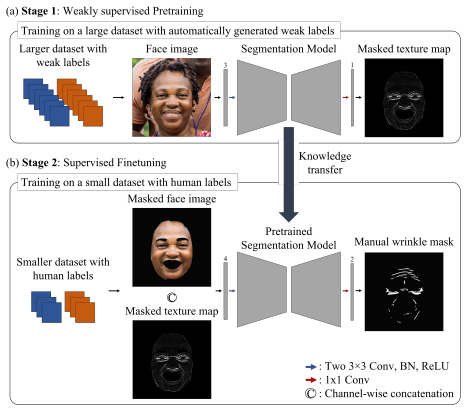
\includegraphics[width=1\textwidth]{2/figures/metoart9.png}
		\caption[Entrenamiento en dos etapas para la segmentación de arrugas faciales]{Entrenamiento en dos etapas para la segmentación de arrugas faciales.\\
			Fuente: \cite{moon2024dermatology}. \citetitle{moon2024dermatology}. (p. 3)}
		\label{2:fig11}
	\end{center}
\end{figure}

\textbf{Base de datos utilizada:}
El estudio introduce el conjunto FFHQ-Wrinkle, derivado del conjunto de datos FFHQ, compuesto por 50,000 imágenes con etiquetas débiles generadas automáticamente y 1,000 imágenes con anotaciones manuales precisas. Este conjunto incluye una amplia variedad de edades, géneros y etnias, lo que contribuye a la robustez del modelo entrenado y favorece su aplicación generalizada en diversos contextos.

\textbf{Resultados:}
Los modelos entrenados mediante la estrategia propuesta lograron un rendimiento superior en comparación con métodos anteriores, tanto en métricas cuantitativas como cualitativas. La combinación de datos etiquetados automáticamente y manualmente permitió reducir significativamente los recursos necesarios para el etiquetado, manteniendo una alta precisión en la segmentación de arrugas faciales, especialmente en regiones clave del rostro.

\textbf{Conclusiones:}
La investigación demuestra que la combinación de aprendizaje débilmente supervisado con ajuste fino supervisado mejora sustancialmente la segmentación automática de arrugas faciales. Además, el nuevo conjunto de datos FFHQ-Wrinkle representa un aporte valioso al campo, ya que ofrece una base estandarizada y diversa para futuras investigaciones sobre análisis facial automatizado y aplicaciones en dermatología estética.
